% This is a Basic Assignment Paper but with like Code and stuff allowed in it, there is also url, hyperlinks from contents included. 

\documentclass[11pt]{article}

% Preamble

\usepackage[margin=1in]{geometry}
\usepackage{amsfonts, amsmath, amssymb}
\usepackage{fancyhdr, float, graphicx}
\usepackage[utf8]{inputenc} % Required for inputting international characters
\usepackage[T1]{fontenc} % Output font encoding for international characters
\usepackage{fouriernc} % Use the New Century Schoolbook font
\usepackage[nottoc, notlot, notlof]{tocbibind}
\usepackage{listings}
\usepackage{xcolor}
\usepackage{blindtext}
\usepackage{hyperref}
\hypersetup{
    colorlinks=true,
    linkcolor=black,
    filecolor=magenta,      
    urlcolor=cyan,
    pdfpagemode=FullScreen,
    }

\definecolor{codegreen}{rgb}{0,0.6,0}
\definecolor{codegray}{rgb}{0.5,0.5,0.5}
\definecolor{codepurple}{rgb}{0.58,0,0.82}
\definecolor{backcolour}{rgb}{0.95,0.95,0.92}

\lstdefinestyle{mystyle}{
    backgroundcolor=\color{backcolour},   
    commentstyle=\color{codegreen},
    keywordstyle=\color{magenta},
    numberstyle=\tiny\color{codegray},
    stringstyle=\color{codepurple},
    basicstyle=\ttfamily\footnotesize,
    breakatwhitespace=false,         
    breaklines=true,                 
    captionpos=b,                    
    keepspaces=true,                 
    numbers=left,                    
    numbersep=5pt,                  
    showspaces=false,                
    showstringspaces=false,
    showtabs=false,                  
    tabsize=2
}

\lstset{style=mystyle}

% Header and Footer
\pagestyle{fancy}
\fancyhead{}
\fancyfoot{}
\fancyhead[L]{\textit{\Large{Internet of Things Lab Assignment 1}}}
\fancyhead[R]{\textit{\Large{Krishnaraj}}}
\fancyfoot[C]{\thepage}
\renewcommand{\footrulewidth}{1pt}



% Other Doc Editing
% \parindent 0ex
%\renewcommand{\baselinestretch}{1.5}

\begin{document}

\begin{titlepage}
	\centering

	%---------------------------NAMES-------------------------------

	\huge\textsc{
		MIT World Peace University
	}\\

	\vspace{0.75\baselineskip} % space after Uni Name

	\LARGE{
		Internet of Things\\
		Second Year B. Tech, Semester 2
	}

	\vfill % space after Sub Name

	%--------------------------TITLE-------------------------------

	\rule{\textwidth}{1.6pt}\vspace*{-\baselineskip}\vspace*{2pt}
	\rule{\textwidth}{0.6pt}
	\vspace{0.75\baselineskip} % Whitespace above the title



	\huge{\textsc{
			Arudino and Raspberry Pi
		}} \\



	\vspace{0.5\baselineskip} % Whitespace below the title
	\rule{\textwidth}{0.6pt}\vspace*{-\baselineskip}\vspace*{2.8pt}
	\rule{\textwidth}{1.6pt}

	\vspace{1\baselineskip} % Whitespace after the title block

	%--------------------------SUBTITLE --------------------------	

	\LARGE\textsc{
		Assignment 1
	} % Subtitle or further description
	\vfill

	%--------------------------AUTHOR-------------------------------

	Prepared By
	\vspace{0.5\baselineskip} % Whitespace before the editors

	\Large{
		Krishnaraj Thadesar \\
		Cyber Security and Forensics\\
		Batch A2, PA 20
	}


	\vspace{0.5\baselineskip} % Whitespace below the editor list
	\today

\end{titlepage}


\tableofcontents
\thispagestyle{empty}
\clearpage

\setcounter{page}{1}

\section{Aim}
To learn about Arduino UNO, and Raspberry Pi Model 3B in detail and thier applications in IoT.

\section{Objectives}
\begin{itemize}
	\item To learn about Arduino UNO and Raspberry Pi Model 3B.
	\item To learn about the applications of Arduino UNO and Raspberry Pi Model 3B in IoT.
\end{itemize}


\section{Equipments Required}
\begin{enumerate}
	\item Raspberry Pi 3 Model
	\item Arduino Uno
	\item Breadboard
	\item Jumper wires
	\item LED
	\item Resistor
\end{enumerate}


\section{Theory}


\subsection{Raspberry Pi Model 3B}

Raspberry Pi Model 3B is a popular single-board computer developed by the Raspberry Pi Foundation. It is a successor to the Raspberry Pi 2 Model B and features a quad-core ARM Cortex-A53 CPU with 1GB of RAM. The board has a variety of input/output options, including HDMI, USB, Ethernet, and a 40-pin GPIO (General Purpose Input/Output) header. \\

It can run various operating systems, including Raspbian, Ubuntu, and Windows 10 IoT Core. Raspberry Pi 3B is used in a variety of projects, including home automation, robotics, and media centers.\\

\subsection{Arduino Uno}
On the other hand, Arduino Uno is a microcontroller board based on the ATmega328P microcontroller. It has 14 digital input/output pins, 6 analog inputs, a 16 MHz quartz crystal, a USB connection, a power jack, and an ICSP header.\\

It can be powered using a USB cable or an external power source. Arduino Uno can be programmed using the Arduino IDE, which supports a variety of programming languages, including C and C++. \\

It is commonly used in various projects, including home automation, robotics, and IoT applications.

\subsection{Difference between Raspberry Pi 3B and Arduino Uno}

One of the main differences between Raspberry Pi 3B and Arduino Uno is their architecture. Raspberry Pi is a full-fledged computer that can run an operating system, while Arduino Uno is a microcontroller board that runs a single program. \\

This makes Raspberry Pi more suitable for projects that require more processing power, such as media centers or web servers. Arduino Uno, on the other hand, is more suitable for projects that require real-time control, such as robotics or home automation.\\



Another difference between the two is their input/output capabilities. Raspberry Pi 3B has a variety of input/output options, including HDMI, USB, Ethernet, and a 40-pin GPIO header, making it suitable for a wide range of projects. Arduino Uno, on the other hand, has a smaller number of input/output pins, making it suitable for simpler projects that require fewer inputs/outputs.\\



In terms of the Internet of Things (IoT), both Raspberry Pi 3B and Arduino Uno can be used to create IoT applications. Raspberry Pi 3B can be used as a web server, which can be accessed remotely over the Internet. \\

It can also be used to interface with various sensors and actuators, making it suitable for IoT applications. Arduino Uno, on the other hand, can be used to create standalone IoT devices that can communicate with other devices over the Internet. \\

It can also be used to interface with various sensors and actuators, making it suitable for a wide range of IoT applications.


\section{Platform}
\textbf{Operating System}: Arch Linux x86-64 \\
\textbf{IDEs or Text Editors Used}: Arduino IDE, and Thonny on Pi\\
\textbf{Compilers} : g++ and gcc on linux for C++, Python 3.10 on Pi\\

\section{Arduino Uno}
\begin{figure}[H]
	\centering
	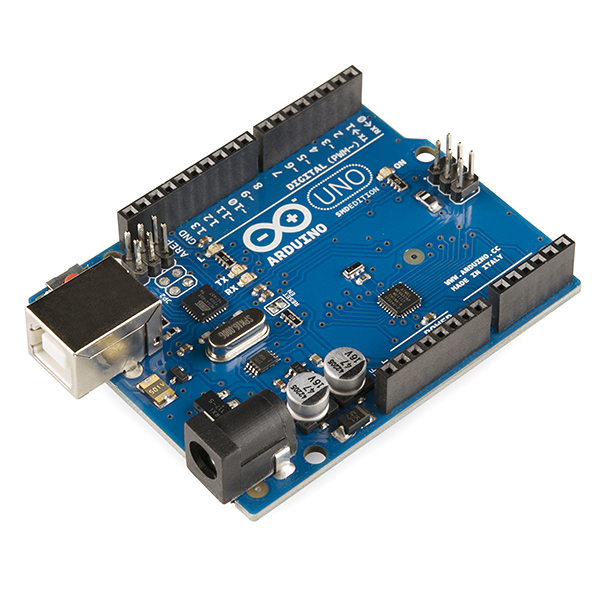
\includegraphics[width=.45\textwidth]{Arduino_Uno_-_R3.jpg}
	\caption{Tinkercad Circuit}
\end{figure}
\section{Arduino Uno Pin Diagram}
\begin{figure}[H]
	\centering
	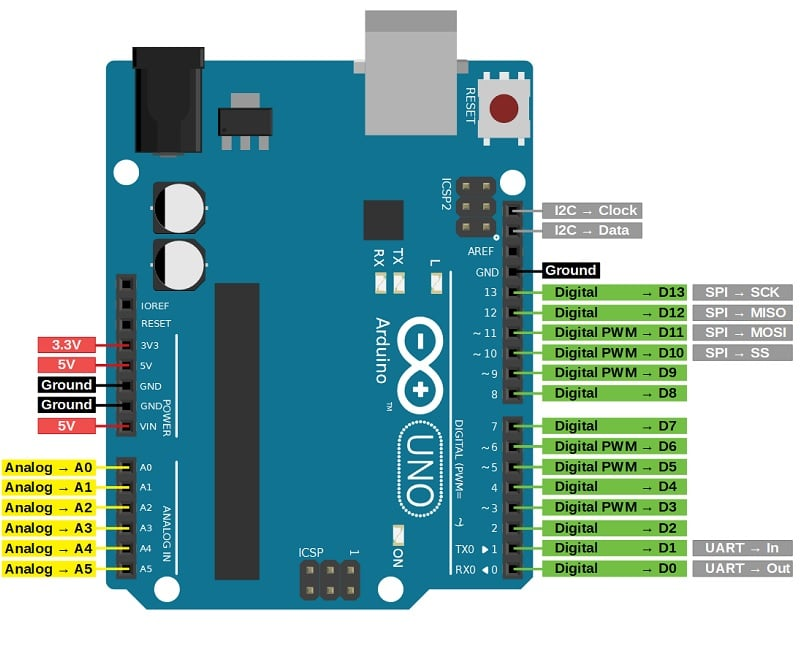
\includegraphics[width=.55\textwidth]{1-3.jpg}
	\caption{Arduino Uno Pin Diagram}
\end{figure}

\section{Raspberry Pi 3B}

\begin{figure}[H]
	\centering
	\includegraphics[width=.75\textwidth]{Raspberry_Pi_4_Model_B_-_Side.jpg}
	\caption{Circuit Diagram}
\end{figure}

\section{Raspberry Pi 3B Pin Diagram}

\begin{figure}[H]
	\centering
	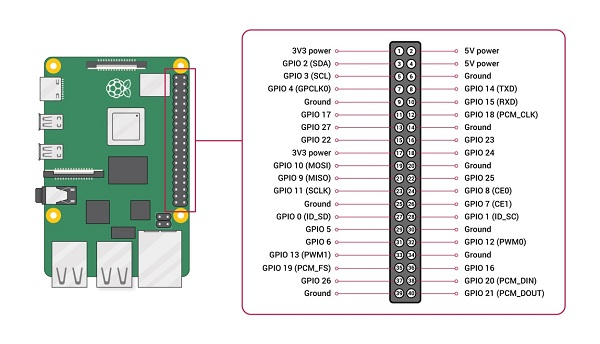
\includegraphics[width=.75\textwidth]{gpio_pinout.jpg}
	\caption{Circuit Diagram}
\end{figure}

\section{Conclusion}
Thus, we have successfully interfaced Temperature Sensor with Arduino Uno and displayed the output on the Serial Monitor.
\clearpage

\section{FAQ}
\begin{enumerate}
	\item Arduino Uno R3 (Code: U1)
	      \begin{itemize}
		      \item Type: Microcontroller board
		      \item Digital pins: 14
		      \item Analog input pins: 6
		      \item Operating voltage: 5V
		      \item Input voltage (recommended): 7-12V
		      \item Input voltage (limits): 6-20V
		      \item Flash memory: 32 KB (ATmega328P microcontroller)
		      \item SRAM: 2 KB (ATmega328P microcontroller)
		      \item EEPROM: 1 KB (ATmega328P microcontroller)
		      \item Clock speed: 16 MHz (ATmega328P microcontroller)
	      \end{itemize}
	\item Raspberry Pi Model 3 B: \\
	      The Raspberry Pi has a total of 40 pins, including 26 GPIO (General Purpose Input/Output) pins, 3.3V and 5V power pins, and ground pins. The pinout diagram for the Raspberry Pi 3 B can be found on the official Raspberry Pi website.

	      \begin{itemize}
		      \item Pin 1: 3.3V
		      \item Pin 2: 5V
		      \item Pin 3: GPIO 2
		      \item Pin 4: 5V
		      \item Pin 5: GPIO 3
		      \item Pin 6: Ground
		      \item Pin 7: GPIO 4
		      \item Pin 8: GPIO 14
		      \item Pin 9: Ground
		      \item Pin 10: GPIO 15
		      \item Pin 11: GPIO 17
		      \item Pin 12: GPIO 18
		      \item Pin 13: GPIO 27
		      \item Pin 14: Ground
		      \item Pin 15: GPIO 22
		      \item Pin 16: GPIO 23
		      \item Pin 17: 3.3V
		      \item Pin 18: GPIO 24
		      \item Pin 19: GPIO 10
		      \item Pin 20: Ground
		      \item Pin 21: GPIO 9
		      \item Pin 22: GPIO 25
		      \item Pin 23: GPIO 11
		      \item Pin 24: GPIO 8
		      \item Pin 25: Ground
		      \item Pin 26: GPIO 7
		      \item Pin 27: ID SD
		      \item Pin 28: ID SC
		      \item Pin 29: GPIO 5
		      \item Pin 30: Ground
		      \item Pin 31: GPIO 6
		      \item Pin 32: GPIO 12
		      \item Pin 33: GPIO 13
		      \item Pin 34: Ground
		      \item Pin 35: GPIO 19
		      \item Pin 36: GPIO 16
		      \item Pin 37: GPIO 26
		      \item Pin 38: GPIO 20
		      \item Pin 39: Ground
		      \item Pin 40: GPIO 21
	      \end{itemize}
\end{enumerate}


\end{document}